\section{Linearization}\label{sec:linearization}
Now that a model of the Cubli frame is put forth in \eqref{finalFrame}, it is apparent that the system is nonlinear due to the term including \si{sin(\theta_F)}. In order to proceed with a simulation and controller design, it is convenient to first linearize the model. This is done by use of a Taylor series approximation.

Based on \eqref{FrameEq3} the system is described in an operating point, around which it varies with \si{\Delta \theta_F}.
%
\begin{flalign}
	\si{(J_F+m_w \cdot {l_w}^{2}) (\ddot{\theta}_{F_0} + \Delta \ddot{\theta}_F )} &= \si{- B_F \cdot (\dot{\theta}_{F_0} + \Delta \dot{\theta}_F) }   \nonumber\\
	&\ \ \ \ \si{+ (m_F \cdot l_F + m_w \cdot l_w) \cdot g \cdot sin(\theta_{F_0} + \Delta \theta_F)} \nonumber\\
	&\ \ \ \ \si{- (\tau_{m_0} + \Delta \tau_m) + B_w \cdot (\dot{\theta}_{w_0} +\Delta \dot{\theta}_w)}  \unit{N \cdot m}\\
	\eq{(J_F+m_w \cdot {l_w}^{2}) (\ddot{\theta}_{F_0} + \Delta \ddot{\theta}_F )}{ f( (\dot{\theta}_{F_0} + \Delta \dot{\theta}_F), \ (\theta_{F_0} + \Delta \theta_F), \ (\tau_{m_0} + \Delta \tau_m),\  (\dot{\theta}_{w_0} + \Delta \dot{\theta}_w) ) } \unit{N \cdot m}
\label{FrameEq4OperatingPoint}
\end{flalign}
%
%The operating point is chosen to be \si{\theta_F = 0}, which corresponds to the frame being in upright position, see \figref{cubliMechanical}.
The operating point is chosen as \si{\theta_{F_0}} and \si{\theta_{w_0}} and their derivatives being equal to 0. This corresponds to the frame being in the upright position, see \figref{cubliMechanical}. At this position all the velocities and accelerations are 0, which results in 0 torque \si{\tau_m} as well.
Taking this into account and applying the Taylor series approximation yields the following.
%
\begin{flalign}
	\si{(J_F+m_w \cdot {l_w}^{2}) \Delta \ddot{\theta}_F } &= \cancelto{0}{\si{f( \dot{\theta}_{F_0}, \ \theta_{F_0}, \ \tau_{m_0},\ \ddot{\theta}_{w_0} )}}   \nonumber\\
	&\ \ \ \ \si{+ \frac{\partial}{\partial \dot{\theta}_F} f\cdot \Delta \dot{\theta}_F + \frac{\partial}{\partial \theta_F} f\cdot \Delta \theta_F + \frac{\partial}{\partial \tau_m} f\cdot \Delta \tau_m + \frac{\partial}{\partial \dot{\theta}_w} f\cdot \Delta \dot{\theta}_w} \unit{N \cdot m}
\label{FrameEq4OperatingPointZero}
\end{flalign}

All the higher order terms are discarded due to their negligible impact on the system when it is near the operating point.
%
\begin{flalign}
	\si{(J_F+m_w \cdot {l_w}^{2}) \Delta \ddot{\theta}_F } &= \si{-B_F \Delta \dot{\theta}_F +  ( m_F \cdot l_F + m_w \cdot l_w ) \cdot g \cdot} \si{  cos(\theta_F)} \si{\Delta \theta_F} \where{\theta_F = 0} \nonumber\\
	&\ \ \ \ \si{- \Delta \tau_m + B_w \Delta \dot{\theta}_w } \unit{N \cdot m}\\
	\eq{(J_F+m_w \cdot {l_w}^{2}) \Delta \ddot{\theta}_F }{-B_F \Delta \dot{\theta}_F +  ( m_F \cdot l_F + m_w \cdot l_w ) \cdot g \cdot \Delta \theta_F - \Delta \tau_m + B_w \Delta \dot{\theta}_w } \unit{N \cdot m}
\label{FrameEq4TaylerApprox}
\end{flalign}
%
\Eqref{FrameEq4TaylerApprox} shows the final linearized model.

%\begin{figure}[H] 
%	\centering 
%	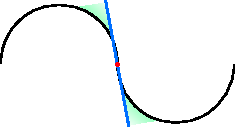
\includegraphics[scale=1.5]{figures/linearizationPoint}
%	\caption{Sketch of linearization for the Cubli frame angels.}
%	\label{LinearizationSketch}
%\end{figure} 
%
%Due to the linearization of the model there will be an point where the controller will no longer be able to catch the frame, because the linear model does not work anymore. In the sketch (see \figref{LinearizationSketch}) the area of operation for the controller is indicated by the green area. 